% =====================================================================
% AGENTRUN 2.0 --- Master manuscript (venue-neutral)
% Compile: pdflatex manuscript.tex ; bibtex manuscript ; pdflatex manuscript.tex ; pdflatex manuscript.tex
% =====================================================================
\documentclass[10pt,twocolumn]{article}

\usepackage[a4paper,margin=2cm]{geometry}
\usepackage{times}
\usepackage{amsmath,amssymb}
\usepackage{booktabs}
\usepackage{graphicx}
\usepackage{xcolor}
\usepackage{tikz}
\usetikzlibrary{arrows.meta,positioning,shapes.geometric}
\usepackage{pgfplots}
\pgfplotsset{compat=1.17}
\usepackage[round,authoryear]{natbib}
\usepackage[hidelinks]{hyperref}

\newcommand{\code}[1]{\texttt{#1}}

\title{\bfseries Disentangling Parser and Data Effects in Tool-Using LLM Fine-Tuning:\\ A Controlled Ablation on Qwen2.5-7B}

\author{
  Alyssa L\\
  \small Department of Information Science and Engineering\\
  \small Siddaganga Institute of Technology, Tumakuru, Karnataka, India\\
  \small \texttt{alyssal282006@gmail.com}
}

\date{}

\begin{document}
\maketitle

\begin{abstract}
\noindent
End-to-end benchmark scores for tool-using language-model agents conflate model capability, training data, and serving-layer infrastructure. We report a controlled ablation that isolates one such confound on a fixed 23-task, machine-checkable multi-tool benchmark. Beginning from an untuned Qwen2.5-7B-Instruct baseline of 22/23 (95.7\%), QLoRA fine-tuning on 35 hand-curated trajectories (condition \textbf{V1}) regressed performance to 18/23 (78.3\%). Trace-level inspection identified two distinct contributing causes: a brittle single-pass tool-call parser that silently discarded malformed model output, and thin training coverage of multi-step, chained, and error-handling tool-use patterns. We then constructed a controlled ablation (condition \textbf{E4}) that evaluates the \emph{V1 adapter unchanged} behind the \emph{corrected two-pass parser}. E4 also scores 18/23 (78.3\%). Thus, on this benchmark, the parser correction produced \emph{zero net aggregate improvement} while changing the per-task composition of failures: two tasks were recovered (\code{multi\_three\_tools}, \code{adversarial\_false\_premise}) and two were newly lost (\code{multi\_search\_weather}, \code{adversarial\_chained\_search\_calc}). A subsequent intervention (condition \textbf{V2}) retained the corrected parser and added 11 targeted trajectories for the specific failure modes observed under V1, recovering all five remaining failures to reach 23/23. We interpret the V1$\to$E4 comparison as a clean estimate of the parser effect on this benchmark (0 net tasks) and the E4$\to$V2 comparison as an observation about targeted augmentation rather than as a randomized causal estimate, because the added trajectories were selected using knowledge of V1's failures. We make no generalization claim beyond the evaluated benchmark. We release all training trajectories, serving code, benchmark definitions, and result artifacts.
\end{abstract}

\noindent\textbf{Keywords:} tool use, function calling, QLoRA, fine-tuning regression, ablation study, parser reliability, agent evaluation, benchmark adaptation.

\section{Introduction}

Large language models (LLMs) are increasingly deployed as agents that select tools, emit structured calls, receive tool outputs, and continue reasoning. The end-to-end score reported by any such system is a composite of many stages: prompt construction, model decoding, serialization of the tool call, extraction by a serving-layer parser, execution by the tool, and finally interpretation of the returned observation by the same model. When a benchmark score changes after an intervention---fine-tuning, prompt editing, parser change, or tool change---the aggregate number alone does not reveal which stage was responsible.

This paper documents a concrete instance of that confound in a small, controlled setting. We fine-tuned Qwen2.5-7B-Instruct with QLoRA~\citep{dettmers2023qlora} on 35 hand-curated tool-use trajectories and observed a regression from the untuned baseline of 22/23 to 18/23 on a fixed 23-task benchmark. Trace-level inspection suggested two candidate causes: (i) a single-pass regex parser that could silently drop malformed but semantically correct tool calls, and (ii) insufficient training coverage of chained tool use, multi-tool synthesis, and error handling.

We then replaced the parser (holding the fine-tuned adapter and training data fixed) and re-evaluated. The resulting condition, \textbf{E4}, scores 18/23: identical to V1 in aggregate but composed of a different set of per-task outcomes. Replacing the parser alone recovered two tasks and broke two others. A subsequent condition, \textbf{V2}, retained the corrected parser and added 11 targeted training trajectories, achieving 23/23.

Our contributions are:
\begin{enumerate}\itemsep2pt
\item A controlled parser ablation (E4) that holds the adapter and training data fixed and varies only the serving-layer parser, providing a clean per-task and aggregate estimate of the parser's effect on the evaluated benchmark.
\item A demonstration that aggregate accuracy can be invariant while failure composition changes: two tasks recovered and two tasks regressed under the parser change.
\item An honest, reproducible record of a fine-tuning regression, its trace-level diagnosis, and a subsequent intervention, with the iterative nature of benchmark development disclosed.
\item An open artifact package containing the training trajectories, serving code for both parsers, the 23-task benchmark, the scoring harness, and all result files.
\end{enumerate}

We deliberately avoid claiming that fine-tuning helped, that the parser mattered in general, or that 23/23 implies generalization. The contribution is methodological and empirical within a small, clearly bounded setting.

\section{Research Questions and Problem Formulation}

\subsection{Problem formulation}

Consider a tool-using agent that, given a user task $x$, produces a sequence of turns. At each turn $t$, the model emits an output string $y_t$ which may contain one or more tool calls. A parser $P$ maps $y_t$ to a set of structured calls $C_t = P(y_t)$. Each call is dispatched to a tool; the tool returns an observation $o_t$; the observation is appended to the model's context; and the loop continues until the model emits a final answer or a step budget $S$ is exhausted.

A benchmark task $i$ defines a required tool set $R_i$, a set of content or numeric predicates on the final answer, and possibly a constraint that a tool error must (or must not) occur. Let $\mathrm{score}_i \in \{0,1\}$ denote the harness's verdict on task $i$ under parser $P$ and adapter $A$. The aggregate accuracy is
\begin{equation}
\mathrm{Acc}(A, P) = \frac{1}{N}\sum_{i=1}^{N}\mathrm{score}_i(A,P).
\end{equation}
We are interested in the contrast between two configurations that share an adapter but differ in parser:
\begin{equation}
\Delta_{\mathrm{parser}}(A) = \mathrm{Acc}(A, P_{V2}) - \mathrm{Acc}(A, P_{V1}).
\end{equation}
The design in this paper estimates $\Delta_{\mathrm{parser}}$ for the specific adapter $A_{V1}$ trained on 35 trajectories. This is the E4 comparison. A separate contrast,
\begin{equation}
\Delta_{\mathrm{data}} = \mathrm{Acc}(A_{V2}, P_{V2}) - \mathrm{Acc}(A_{V1}, P_{V2}),
\end{equation}
measures the combined effect of changing the adapter and adding 11 targeted trajectories, holding the parser fixed. This is the E4$\to$V2 comparison. The second contrast is \emph{not} a randomized causal estimate: the added trajectories were authored using knowledge of V1's failures.

\subsection{Research questions}

\noindent\textbf{RQ1.} On a fixed benchmark, what is the net aggregate effect of replacing the V1 parser with the V2 two-pass parser while holding the V1 adapter and training data constant?

\noindent\textbf{RQ2.} Does that replacement change the composition of per-task failures even when the aggregate does not change?

\noindent\textbf{RQ3.} What is the observed change when targeted trajectories are added after the parser replacement, and what are the validity conditions under which that change can be interpreted?

\noindent\textbf{RQ4.} Which of these results can be generalized beyond the evaluated benchmark, and which cannot?

\section{Related Work}

We organize prior work into five threads that bear directly on this study.

\subsection{Tool-using and function-calling language models}

ReAct~\citep{yao2022react} established the interleaved reason--act--observe loop that motivates most modern agent designs. Toolformer~\citep{schick2023toolformer} showed that a language model can self-supervise the placement of API calls via a generate-and-filter procedure. Gorilla~\citep{patil2023gorilla} fine-tuned LLaMA-7B for accurate invocation across 1,600+ APIs using retrieval. ToolLLM~\citep{qin2023toolllm} scaled demonstration data to 16{,}000+ APIs via depth-first search over tool compositions. API-Bank~\citep{li2023apibank} introduced a benchmark of 11{,}428 samples across 53 APIs, explicitly separating API selection from argument generation.

These works established both the capability and the evaluation landscape but largely assume a correct parser between model output and tool execution. Our study treats the parser as part of the evaluated system.

\subsection{Agent evaluation}

AgentBench~\citep{liu2023agentbench} evaluates LLM agents across 11 interactive environments. WebArena~\citep{zhou2023webarena} evaluates agents on realistic web tasks. Common to these benchmarks is an end-to-end aggregate score that does not, in itself, decompose model-level errors from serving-layer or protocol-level errors.

Our benchmark is far smaller (23 tasks, single tool surface) and its purpose is orthogonal: to permit exhaustive trace-level attribution of every failure, at the cost of statistical strength.

\subsection{Agent fine-tuning}

FireAct~\citep{chen2023fireact} fine-tuned language agents on ReAct-style trajectories and reported improvements on HotpotQA and ALFWorld. AgentTuning~\citep{zeng2023agenttuning} curated 37k multi-turn trajectories and showed gains on held-out agent tasks. These works demonstrate that fine-tuning can improve agent behavior at scale. They do not typically report controlled ablations that hold the adapter fixed while varying serving infrastructure.

Our study operates at a much smaller data scale (35 and 46 trajectories) and focuses on failure dynamics rather than scaling laws.

\subsection{Parameter-efficient fine-tuning}

LoRA~\citep{hu2021lora} and QLoRA~\citep{dettmers2023qlora} make 7B-scale fine-tuning feasible on a single consumer or free-tier GPU. We use a shared QLoRA configuration across conditions, so that the differences we observe are confined to the adapter, the training data, and the parser---with one exception we state explicitly in Section~\ref{sec:setup}, namely three memory-related optimizer settings that the V2 training script adds.

\subsection{Evaluation reliability, structured output, and benchmark adaptation}

\textbf{Structured generation.} Willard and Louf~\citep{willard2023guided} proposed finite-state-machine-guided generation for structured output. Related work treats the reliability of serializing structured model output as a first-class engineering problem. Our parser is a lightweight, hand-written alternative to constrained decoding and has known failure modes we characterize.

\textbf{Contamination and adaptive evaluation.} \citet{sainz2023contamination} and \citet{deng2023contamination} documented the ways in which benchmark results can be inflated by data contamination or by iterative benchmark development. Our study is not contaminated in the classical sense---no benchmark prompt appears in the training data---but the V2 augmentation was authored with knowledge of which benchmark tasks V1 failed. This is a mild form of evaluation adaptation, and we disclose it explicitly.

\subsection{Positioning}

To our knowledge, no prior study on this scale has reported a controlled ablation in which the serving-layer tool-call parser is varied while the adapter and training data are held fixed, with per-task outcomes reported alongside the aggregate.

\section{The AGENTRUN System}

\subsection{Pipeline}

Figure~\ref{fig:pipeline} shows the AGENTRUN pipeline. The model emits output $y_t$, the parser extracts tool calls $C_t$, the executor runs them, the observations $o_t$ are appended to the context, and the loop repeats until a final answer or the step budget is exhausted.

\begin{figure}[t]
\centering
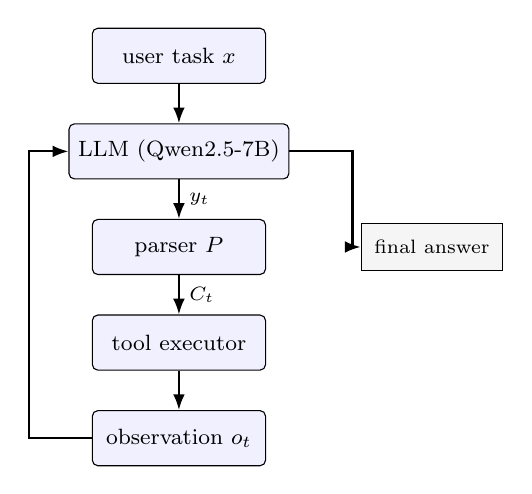
\begin{tikzpicture}[
  node distance=5mm,
  box/.style={rectangle, rounded corners=2pt, draw, fill=blue!6, minimum width=22mm, minimum height=7mm, align=center, font=\footnotesize},
  small/.style={rectangle, draw, fill=gray!8, minimum width=18mm, minimum height=6mm, align=center, font=\scriptsize},
  arr/.style={-{Latex[length=2mm]}, thick}
]
\node[box] (task) {user task $x$};
\node[box, below=of task] (llm) {LLM (Qwen2.5-7B)};
\node[box, below=of llm] (parser) {parser $P$};
\node[box, below=of parser] (exec) {tool executor};
\node[box, below=of exec] (obs) {observation $o_t$};
\node[small, right=12mm of parser] (ans) {final answer};
\draw[arr] (task) -- (llm);
\draw[arr] (llm) -- node[right,font=\scriptsize]{$y_t$} (parser);
\draw[arr] (parser) -- node[right,font=\scriptsize]{$C_t$} (exec);
\draw[arr] (exec) -- (obs);
\draw[arr] (obs.west) -- ++(-8mm,0) |- (llm.west);
\draw[arr] (llm.east) -- ++(8mm,0) |- (ans.west);
\end{tikzpicture}
\caption{The AGENTRUN pipeline. The parser sits between model output and tool execution; failures at the parser stage are indistinguishable at the aggregate score from failures at the model or tool stages.}
\label{fig:pipeline}
\end{figure}

\subsection{Model and adapters}

The base model is \code{Qwen/Qwen2.5-7B-Instruct}~\citep{qwen2024qwen} (7.6B parameters), served in 4-bit NF4 quantization with fp16 compute. LoRA adapters are applied with rank $r=16$, $\alpha=16$, dropout $0.05$, target modules $\{\code{q\_proj}, \code{k\_proj}, \code{v\_proj}, \code{o\_proj}\}$. Two adapters exist:
\begin{itemize}\itemsep2pt
\item \textbf{V1}: trained on 35 hand-curated trajectories.
\item \textbf{V2}: trained on 46 trajectories, i.e., the V1 set plus 11 targeted trajectories.
\end{itemize}
Both adapters share the same LoRA, data, and optimization hyperparameters; the
three memory-related settings that differ are listed in Table~\ref{tab:train}.

\subsection{Tool surface}

The tool surface is fixed across all conditions and consists of exactly four tools: \code{calculator}, \code{word\_count}, \code{web\_search} (Tavily API), and \code{get\_weather} (Open-Meteo). Tool calls are transported via a Model Context Protocol server over stdio. The tool surface and tool schemas presented to the model are byte-identical across all conditions; only the model and the parser vary.

\subsection{Parser variants}

Two parsers are used. Both consume the raw string output of the model and return a dictionary \code{\{"tool\_calls": [...], "text": ...\}}.

\paragraph{V1 parser (single-pass).} A single regular expression matches properly closed \code{<tool\_call>}\ldots\code{</tool\_call>} blocks:
\begin{quote}\footnotesize\ttfamily
TOOL\_CALL\_PATTERN = re.compile(\\
\hspace*{1em}r"<tool\_call>\textbackslash s*(\{\textbackslash .*?\})\textbackslash s*</tool\_call>", re.DOTALL)
\end{quote}
If the model emits a malformed block---e.g., an unclosed opening tag followed by a second opening tag---the regex's non-greedy match spans across the malformed boundary, fails to parse the captured substring as JSON, and returns no tool calls. The server then treats the entire raw output as a final answer.

\paragraph{V2 parser (two-pass).} A first pass attempts strict matching, identical to V1. If the strict pass finds nothing, a second pass extracts the first JSON object occurring after any \code{<tool\_call>} opening tag. The second pass has a known limitation: it can only recover the \emph{first} tool call when the model emits multiple malformed blocks in a single turn, and it may truncate arguments that contain nested JSON.

\subsection{Experimental conditions}

Four conditions are compared (Table~\ref{tab:matrix}).

\begin{table}[t]
\centering
\caption{Experiment matrix. E4 is the controlled parser ablation.}
\label{tab:matrix}
\small
\begin{tabular}{lcccc}
\toprule
ID & Adapter & Training data & Parser & Score \\
\midrule
Base & none     & none             & V1 & 22/23 \\
V1   & V1       & 35 trajectories  & V1 & 18/23 \\
\textbf{E4} & \textbf{V1} & \textbf{35 trajectories} & \textbf{V2} & \textbf{18/23} \\
V2   & V2       & 46 trajectories  & V2 & 23/23 \\
\bottomrule
\end{tabular}
\end{table}

The E4 condition holds the adapter and training data equal to V1, and changes only the parser to the V2 version.

\section{Experimental Setup}
\label{sec:setup}

\subsection{Training configuration}

Table~\ref{tab:train} lists the training configuration of both runs. Every LoRA
and data hyperparameter is shared. Three memory-related settings are not: the V2
script additionally enables gradient checkpointing, disables the KV cache, and
passes a paged 8-bit AdamW optimizer explicitly, because the 46-trajectory run
had to fit in the 15\,GB budget of a free-tier T4. The V1 script does not set
these and therefore uses the \texttt{Trainer} default optimizer. We record the
difference because it does not affect the E4 ablation, which varies only the
parser, but it does mean that the E4$\to$V2 contrast changes the adapter, the
training data, and these optimizer settings simultaneously
(Section~\ref{sec:data}).

\begin{table}[t]
\centering
\caption{Training configuration. All rows are shared between V1 and V2 except
the three memory-related settings, which are added in the V2 script.}
\label{tab:train}
\small
\begin{tabular}{ll}
\toprule
Hyperparameter & Value \\
\midrule
Base model         & \code{Qwen/Qwen2.5-7B-Instruct} \\
Quantization       & 4-bit NF4, fp16 compute \\
LoRA rank $r$      & 16 \\
LoRA $\alpha$      & 16 \\
LoRA dropout       & 0.05 \\
Target modules     & \code{q,k,v,o}\_\code{proj} \\
\midrule
Optimizer          & V1: default; V2: \code{PagedAdamW8bit} \\
Gradient ckpt.     & V1: off; V2: on \\
KV cache           & V1: on; V2: off \\
\midrule
Learning rate      & $2\times10^{-4}$ \\
Per-device batch   & 2 \\
Gradient accum.    & 4 \\
Effective batch    & 8 \\
Epochs             & 3 \\
Max seq. length    & 1024 \\
Hardware           & Colab T4 (15\,GB) \\
\bottomrule
\end{tabular}
\end{table}

\subsection{Training trajectories}

\textbf{V1 (35 trajectories).} Generated by running the untuned base agent over a set of training prompts and retaining only trajectories that completed within the step budget without tool errors. Training prompts are disjoint from benchmark prompts.

\textbf{V2 (46 trajectories).} The V1 set plus 11 targeted additions (Table~\ref{tab:aug}).

\begin{table}[t]
\centering
\caption{V2 targeted augmentation (11 additional trajectories).}
\label{tab:aug}
\small
\begin{tabular}{lc}
\toprule
Targeted gap & Trajectories added \\
\midrule
\code{word\_count} $\to$ \code{calculator} chains & 3 \\
\code{get\_weather} $\to$ \code{calculator} chains & 3 \\
Three-tool chain with final synthesis & 2 \\
Calculator error handling (division by zero) & 2 \\
False-premise identification and correction & 1 \\
\midrule
\textbf{Total} & \textbf{11} \\
\bottomrule
\end{tabular}
\end{table}

The choice of \emph{which} patterns to add was informed by inspecting which benchmark categories V1 failed. This is disclosed and analyzed in Sections~\ref{sec:discussion} and~\ref{sec:threats}.

\subsection{Benchmark}

The benchmark consists of 23 machine-checkable tasks (Table~\ref{tab:cats}).

\begin{table}[t]
\centering
\caption{Benchmark task categories (23 tasks).}
\label{tab:cats}
\small
\begin{tabular}{lcl}
\toprule
Category & \# & What it probes \\
\midrule
\code{math}                       & 3 & Arithmetic, precedence \\
\code{text}                       & 1 & Word counting \\
\code{weather}                    & 2 & Live weather lookup \\
\code{search}                     & 2 & Live web search \\
\code{multi\_tool}                & 4 & Independent tools, one turn \\
\code{chained\_reasoning}         & 1 & Tool $B$ depends on $A$ \\
\code{time\_sensitive}            & 1 & Live info, not parametric \\
\code{no\_tool\_expected}         & 2 & Withholding tool use \\
\code{adversarial\_math}          & 3 & Negatives, decimals, \% \\
\code{adversarial\_reasoning}     & 2 & False premise; chain \\
\code{adversarial\_error\_handling} & 1 & Tool must error (div.) \\
\code{adversarial\_ambiguity}     & 1 & Underspecified entity \\
\midrule
\textbf{Total} & \textbf{23} & \\
\bottomrule
\end{tabular}
\end{table}

Each task's success predicate is checked against the full execution trace: (i) required tools present in the trace's tool-name set, (ii) no unexpected tool error unless the task explicitly requires one, (iii) termination within \code{max\_steps = 3}, and (iv) any content or numeric predicate satisfied by the final answer.

\subsection{Evaluation protocol}

All four conditions were evaluated with the same benchmark, \code{max\_steps = 3}, greedy decoding (\code{do\_sample=False}), and the same tool surface and tool schemas. The Tavily API key was active for all runs; no tool is mocked.

\section{Failure Analysis}

We attribute each of the six discriminating tasks to a mechanism based on trace inspection and the parser design.

\subsection{Parser-recovered tasks}

\paragraph{\code{adversarial\_false\_premise}.} The task requires the model to search for a fictional entity's GDP and explicitly reject the false premise. Under V1, the model emitted a malformed \code{<tool\_call>} block; the single-pass parser dropped the call; the server treated the output as a final answer that failed the required-content predicate. Under E4, the two-pass parser recovered the search call, the tool returned no reliable result, and the model produced a final answer containing the required fictional-premise acknowledgment. \emph{Attribution: parser.}

\paragraph{\code{multi\_three\_tools}.} The task requires three parallel tool calls and a final synthesis. Under V1, the parser dropped one of the three calls, and the model exhausted its step budget before producing a synthesis. Under E4, the two-pass parser recovered the missing call, and the model completed the task within budget. \emph{Attribution: parser.}

\subsection{Parser-regressed tasks}

\paragraph{\code{multi\_search\_weather}.} Under V1, the malformed tool call caused the parser to return no calls; the model answered directly, and the answer happened to satisfy the task's predicates. Under E4, the two-pass parser correctly extracted the \code{web\_search} call; the model then failed to also call \code{get\_weather} in the remaining turns and exhausted the budget. \emph{Attribution: parser-induced change in execution trace.}

\paragraph{\code{adversarial\_chained\_search\_calc}.} Same mechanism. Under V1, the parser's silent failure produced a direct answer that happened to be numerically correct. Under E4, the parser correctly extracted the search call, and the model's subsequent multi-step path exceeded the step budget. \emph{Attribution: parser-induced change in execution trace.}

\subsection{Unchanged failures}

\paragraph{\code{multi\_wordcount\_calc}.} Under both V1 and E4 the model calls \code{word\_count} but performs the multiplication in prose rather than via the calculator. The predicate requires the calculator in the trace. \emph{Attribution: model behavior, not parser.}

\paragraph{\code{chain\_weather\_then\_calc}.} Under both conditions the model calls \code{get\_weather} but computes the Celsius-to-Fahrenheit conversion in text. \emph{Attribution: model behavior, not parser.}

\paragraph{\code{adversarial\_division\_by\_zero}.} The task requires the model to invoke the calculator with a division-by-zero expression and acknowledge the resulting error. Under Base, V1, and E4 the model answers in prose without calling the calculator. \emph{Attribution: model behavior; not recovered by parser change.}

\section{Results}

\begin{table}[t]
\centering
\caption{Aggregate accuracy across conditions.}
\label{tab:agg}
\small
\begin{tabular}{lcccc}
\toprule
Condition & Adapter & Parser & Passed & Accuracy \\
\midrule
Base & none & V1 & 22/23 & 95.7\% \\
V1   & V1 (35) & V1 & 18/23 & 78.3\% \\
\textbf{E4} & \textbf{V1 (35)} & \textbf{V2} & \textbf{18/23} & \textbf{78.3\%} \\
V2   & V2 (46) & V2 & 23/23 & 100.0\% \\
\bottomrule
\end{tabular}
\end{table}

Two decompositions follow directly:
\begin{itemize}\itemsep2pt
\item \textbf{Parser effect:} $\Delta_{\mathrm{parser}}(A_{V1}) = 18/23 - 18/23 = 0$ net tasks.
\item \textbf{Data effect:} $\mathrm{Acc}(A_{V2}, P_{V2}) - \mathrm{Acc}(A_{V1}, P_{V2}) = 23/23 - 18/23 = +5$ tasks.
\end{itemize}

\begin{figure}[t]
\centering
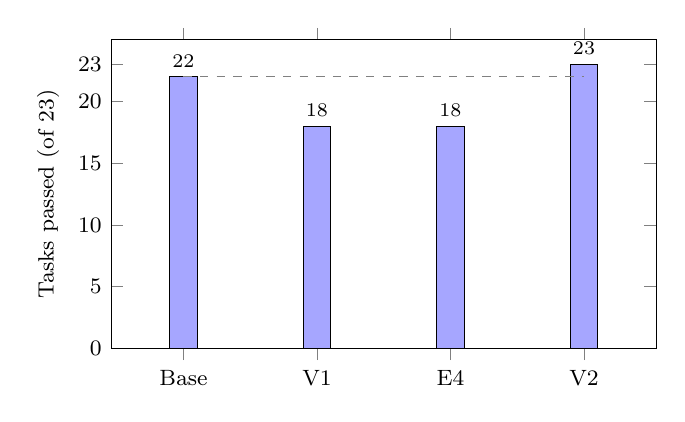
\begin{tikzpicture}[font=\footnotesize]
\begin{axis}[
  ybar, width=8.5cm, height=5.5cm,
  ymin=0, ymax=25,
  ylabel={Tasks passed (of 23)},
  symbolic x coords={Base,V1,E4,V2},
  xtick=data,
  ytick={0,5,10,15,20,23},
  bar width=10pt,
  nodes near coords,
  nodes near coords style={font=\scriptsize},
  enlarge x limits=0.18,
]
\addplot[fill=blue!35] coordinates {(Base,22) (V1,18) (E4,18) (V2,23)};
\draw[dashed,gray] (axis cs:Base,22) -- (axis cs:V2,22);
\end{axis}
\end{tikzpicture}
\caption{Aggregate pass counts. Dashed line marks Base. E4 matches V1 in aggregate; V2 exceeds both.}
\label{fig:results}
\end{figure}

\subsection{Per-task decomposition}

Table~\ref{tab:pertask} reports every benchmark task under all four conditions.

\begin{table*}[t]
\centering
\caption{Per-task outcomes across all conditions. \checkmark~= pass, $\times$~= fail. Columns $\Delta_1$ and $\Delta_2$ record V1$\to$E4 and E4$\to$V2 changes.}
\label{tab:pertask}
\small
\begin{tabular}{llcccccc}
\toprule
Task ID & Category & Base & V1 & E4 & V2 & $\Delta_1$ & $\Delta_2$ \\
\midrule
\code{calc\_basic\_1}                    & math      & \checkmark & \checkmark & \checkmark & \checkmark & -- & -- \\
\code{calc\_basic\_2}                    & math      & \checkmark & \checkmark & \checkmark & \checkmark & -- & -- \\
\code{calc\_order\_of\_ops}              & math      & \checkmark & \checkmark & \checkmark & \checkmark & -- & -- \\
\code{wordcount\_basic}                  & text      & \checkmark & \checkmark & \checkmark & \checkmark & -- & -- \\
\code{weather\_basic\_1}                 & weather   & \checkmark & \checkmark & \checkmark & \checkmark & -- & -- \\
\code{weather\_basic\_2}                 & weather   & \checkmark & \checkmark & \checkmark & \checkmark & -- & -- \\
\code{search\_basic\_1}                  & search    & \checkmark & \checkmark & \checkmark & \checkmark & -- & -- \\
\code{search\_basic\_2}                  & search    & \checkmark & \checkmark & \checkmark & \checkmark & -- & -- \\
\code{multi\_weather\_calc}              & multi     & \checkmark & \checkmark & \checkmark & \checkmark & -- & -- \\
\code{multi\_wordcount\_calc}            & multi     & \checkmark & $\times$   & $\times$   & \checkmark & -- & $+1$ \\
\code{multi\_search\_weather}            & multi     & \checkmark & \checkmark & $\times$   & \checkmark & $-1$ & $+1$ \\
\code{multi\_three\_tools}               & multi     & \checkmark & $\times$   & \checkmark & \checkmark & $+1$ & -- \\
\code{chain\_weather\_then\_calc}        & chained   & \checkmark & $\times$   & $\times$   & \checkmark & -- & $+1$ \\
\code{time\_sensitive\_1}                & time      & \checkmark & \checkmark & \checkmark & \checkmark & -- & -- \\
\code{no\_tool\_needed\_1}               & no-tool   & \checkmark & \checkmark & \checkmark & \checkmark & -- & -- \\
\code{no\_tool\_needed\_2}               & no-tool   & \checkmark & \checkmark & \checkmark & \checkmark & -- & -- \\
\code{adversarial\_negative\_multiply}   & adv-math  & \checkmark & \checkmark & \checkmark & \checkmark & -- & -- \\
\code{adversarial\_decimal\_division}    & adv-math  & \checkmark & \checkmark & \checkmark & \checkmark & -- & -- \\
\code{adversarial\_percentage}           & adv-math  & \checkmark & \checkmark & \checkmark & \checkmark & -- & -- \\
\code{adversarial\_false\_premise}       & adv-reas  & \checkmark & $\times$   & \checkmark & \checkmark & $+1$ & -- \\
\code{adversarial\_chained\_search\_calc}& adv-reas  & \checkmark & \checkmark & $\times$   & \checkmark & $-1$ & $+1$ \\
\code{adversarial\_division\_by\_zero}   & adv-err   & $\times$   & $\times$   & $\times$   & \checkmark & -- & $+1$ \\
\code{adversarial\_ambiguous\_city}      & adv-amb   & \checkmark & \checkmark & \checkmark & \checkmark & -- & -- \\
\midrule
\textbf{Passed} & & \textbf{22} & \textbf{18} & \textbf{18} & \textbf{23} & \textbf{0} & \textbf{+5} \\
\bottomrule
\end{tabular}
\end{table*}

\section{Controlled Parser Ablation}
\label{sec:parser}

The V1$\to$E4 comparison is the cleanest evidence in this study.

\begin{quote}
\itshape
On the 23-task benchmark, replacing the V1 single-pass parser with the V2 two-pass parser, while holding the V1 adapter and training data fixed, produced \textbf{zero net change in aggregate accuracy} (18/23 $\to$ 18/23).
\end{quote}

Two observations complicate but do not weaken this result:
\begin{enumerate}\itemsep2pt
\item The parser change did affect specific tasks. Two tasks that V1 failed were recovered; two tasks that V1 passed were regressed.
\item The parser's correct extraction can drive the model down an execution path that happens to exceed the step budget. The \code{multi\_search\_weather} and \code{adversarial\_chained\_search\_calc} regressions are examples.
\end{enumerate}

\begin{figure}[t]
\centering
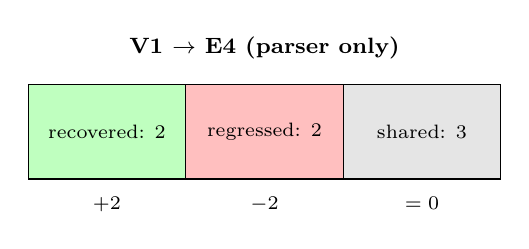
\begin{tikzpicture}[font=\footnotesize, scale=1.0]
\draw[fill=green!25] (0,0) rectangle (2,1.2);
\node at (1,0.6) {\scriptsize recovered: 2};
\draw[fill=red!25] (2,0) rectangle (4,1.2);
\node at (3,0.6) {\scriptsize regressed: 2};
\draw[fill=gray!20] (4,0) rectangle (6,1.2);
\node at (5,0.6) {\scriptsize shared: 3};
\node[below] at (1,-0.1) {\scriptsize $+2$};
\node[below] at (3,-0.1) {\scriptsize $-2$};
\node[below] at (5,-0.1) {\scriptsize $=0$};
\node[above] at (3,1.4) {\textbf{V1 $\to$ E4 (parser only)}};
\end{tikzpicture}
\caption{Per-task transitions under the parser ablation. Recoveries and regressions cancel exactly.}
\label{fig:parser}
\end{figure}

\section{Data-Augmentation Analysis}
\label{sec:data}

The E4$\to$V2 transition retains the corrected parser and changes the adapter from V1 (35 trajectories) to V2 (46 trajectories). It recovers all five E4 failures. We state this as an observation, not as a randomized causal estimate. Four reasons:
\begin{enumerate}\itemsep2pt
\item The 11 additional trajectories were selected because V1 failed on those patterns. This is a form of evaluation adaptation.
\item The adapter change and the training-data change are inseparable here.
\item The V2 training script also enables gradient checkpointing, disables the KV cache, and uses a paged 8-bit optimizer that the V1 script does not (Table~\ref{tab:train}), so the two runs are not separated along the training axis alone.
\item No seeds, no repetitions, and no held-out benchmark are available in this study.
\end{enumerate}

\begin{quote}
\itshape
The defensible statement is: on the evaluated benchmark, retraining on 46 trajectories (the V1 set plus 11 targeted additions) under the corrected parser, with the V2 run's memory-related optimizer settings, coincides with recovery of all five remaining failures. Whether the same intervention would generalize is not tested.
\end{quote}

\begin{figure}[t]
\centering
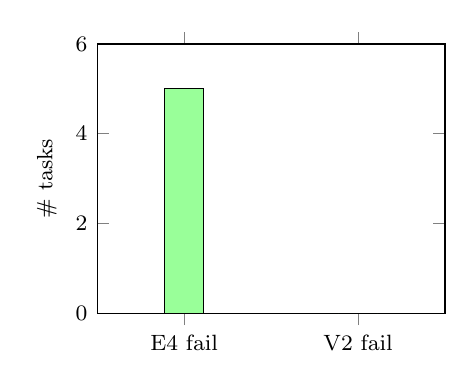
\begin{tikzpicture}[font=\footnotesize]
\begin{axis}[
  ybar, width=6cm, height=5cm,
  ymin=0, ymax=6,
  ylabel={\# tasks},
  symbolic x coords={E4 fail,V2 fail},
  xtick=data,
  bar width=14pt,
  enlarge x limits=0.5,
]
\addplot[fill=green!40] coordinates {(E4 fail,5) (V2 fail,0)};
\end{axis}
\end{tikzpicture}
\caption{E4$\to$V2 transition: all five E4 failures recovered; none regressed.}
\label{fig:decomp}
\end{figure}

\section{Discussion}
\label{sec:discussion}

\subsection{Interpreting the parser ablation}

The E4 result is the cleanest evidence in the study. On the 23-task benchmark, replacing the V1 single-pass parser with the V2 two-pass parser, while holding the V1 adapter and training data fixed, produced zero net change in aggregate accuracy. The parser change did affect specific tasks: two were recovered and two were regressed. The parser's correct extraction can drive the model down an execution path that happens to exceed the step budget.

\subsection{Interpreting the E4$\to$V2 transition}

The E4$\to$V2 transition retains the corrected parser and changes the adapter. It recovers all five E4 failures. We state this as an observation, not as a randomized causal estimate, for the three reasons given in Section~\ref{sec:data}.

\subsection{Aggregate invariance and failure redistribution}

The V1$\to$E4 result illustrates a general point for agent evaluation: an aggregate score can be invariant while the underlying failure composition changes. A deployment decision that treats the two conditions as equivalent because the aggregate is equal would be incorrect if the specific tasks that fail matter.

\subsection{Why fine-tuning can regress}

V1's drop from 22/23 to 18/23 is not fully explained by the parser defect. Of V1's five failures, three persist under the corrected parser in E4. The study does not identify whether this is catastrophic forgetting, overfitting, or a coverage gap; it identifies the patterns that regressed and the training data that did not cover them.

\section{Threats to Validity}
\label{sec:threats}

\textbf{Internal validity.} The E4 comparison is a clean controlled contrast: adapter and training data are fixed; only the parser changes. The E4$\to$V2 comparison is not a clean causal contrast: the added data was authored using knowledge of V1 failures, and the V2 training script additionally changes the optimizer and gradient-checkpointing settings (Table~\ref{tab:train}). Environmental variance from live web search is uncontrolled.

\textbf{External validity.} Results are on a single model family (Qwen2.5-7B-Instruct) and a single 23-task benchmark with four tools. Generalization to other models, benchmarks, or tool surfaces is not tested.

\textbf{Construct validity.} The scoring harness combines multiple stages of behavior into a single binary outcome. Distinguishing ``model failed to select the tool'' from ``model selected the tool but the parser dropped the call'' requires trace inspection that the harness does not perform.

\textbf{Statistical validity.} One run per condition. No variance estimate. No significance test.

\textbf{Evaluation validity.} The 23-task benchmark was used iteratively during development. The V2 augmentation was designed after observing V1's failures. A fresh held-out benchmark is required for a generalization claim; we do not make one.

\textbf{Reproducibility validity.} Python 3.11.9, torch 2.13.0+cpu, transformers 5.15.1, peft 0.20.0, accelerate 1.14.0 are recorded. Colab CUDA and driver versions were not recorded. Random seeds for training and evaluation were not set.

\section{Limitations}

\begin{itemize}\itemsep2pt
\item \textbf{N=1 per condition.} No multi-seed runs. Variance is unknown.
\item \textbf{Single model family.} All results are Qwen2.5-7B-Instruct.
\item \textbf{Small benchmark.} 23 tasks; six categories have N=1.
\item \textbf{Iterative benchmark development.} V2's training data was informed by V1's failures on this exact benchmark.
\item \textbf{No fresh held-out benchmark.} Not run.
\item \textbf{Retraining is not isolated.} The V2 run differs from V1 in training data and in three memory-related optimizer settings; no run isolates the data change on its own.
\item \textbf{Greedy decoding only.}
\item \textbf{Real external-tool variability.}
\item \textbf{E4 trace incompleteness.} E4 result artifacts record pass/fail per task but not the full per-task traces.
\end{itemize}

The 23/23 V2 result means ``23/23 on the evaluated benchmark.'' It does not mean the model generalizes perfectly, that the augmentation caused the improvement in a randomized sense, or that the parser fix mattered in general.

\section{Reproducibility and Artifact Availability}

All artifacts are available at \url{https://github.com/alyssa2ai/AGENTRUN}:
\begin{itemize}\itemsep2pt
\item \code{eval/tasks.py} --- 23-task benchmark definitions.
\item \code{eval/harness.py} --- scoring logic.
\item \code{training/training\_data.jsonl} --- V1 trajectories (35).
\item \code{training/training\_data\_augmented.jsonl} --- V2 trajectories (46).
\item \code{serving/colab\_server.py}, \code{serving/colab\_server\_e4.py}, \code{serving/colab\_server\_v2.py} --- serving code.
\item \code{results/eval\_results\_\{base,v1,e4,v2\}.json} --- raw per-condition results.
\item \code{results/experiment\_summary.json} --- full matrix and provenance.
\item \code{results/verify\_results.py} --- recomputes every reported tally and transition from the committed result files.
\item \code{provenance/experiment\_provenance.json} --- provenance record with per-field verification labels.
\end{itemize}

\textbf{Missing metadata} (flagged rather than guessed): exact Colab CUDA and driver versions; training and evaluation random seeds; exact wall-clock timestamp of the E4 run.

\section{Conclusion}

We presented a controlled ablation of a serving-layer parser in a small tool-using LLM agent. On the evaluated 23-task benchmark, replacing the V1 single-pass parser with a V2 two-pass parser, holding the fine-tuned adapter and training data fixed, produced zero net aggregate improvement while changing the composition of per-task outcomes. A subsequent intervention retained the corrected parser and introduced 11 targeted training trajectories, recovering all five remaining failures. We interpret the first result as a clean estimate of the parser effect on this benchmark and the second as a benchmark-specific observation that does not support a causal or generalizing claim.

Three recommendations follow. First, when multiple changes are made between reported conditions, run a controlled ablation that isolates each change. Second, report per-task outcomes alongside aggregate scores; equal aggregates can hide opposite-sign per-task effects. Third, treat targeted training-data augmentation as a legitimate but not blindly causal intervention; if the augmentation was informed by observed failures on the evaluation set, disclose that.

Future work should include multi-seed evaluation, a fresh held-out benchmark with novel task instances, a random-augmentation control, and cross-model replication. None of these are prerequisites for the claim we make; they are prerequisites for a stronger claim we deliberately do not make.

\bibliographystyle{plainnat}
\bibliography{references}

\end{document}
